% !TEX root = ../main.tex
\section{Summary}
\label{sec:summary}

Bantay-Baha joins three graphs into one ranking: a flood-exposure layer (rain, river routing, observed and mapped flood), a lead-lag outbreak graph learned between provinces, and a road and ferry access graph that a typhoon cuts. A quantile forecast of dengue gives the probability $R$ that a province's next four weeks exceed its usual bad month; two access methods give the share $A$ of people cut off from a hospital; the priority is $P = R \times A$. Dengue forecasting in the Philippines has been studied at province level before \parencite{buczak2014}, and typhoon flooding is followed by leptospirosis \parencite{balbuena2010}; what is new here is the combination with storm-driven access loss, ranked for any typhoon track. Every number in this document was computed by the build (\code{build.bat}) from the raw files and written into it by \code{scripts/make\_spec.py}.

\subsection{Findings}

\begin{itemize}
\item \textbf{The forecast beats the bar.} Multi-quantile XGBoost reaches a relative WIS of \relWISHOne{} at one week and \relWISHFour{} at four weeks over \nScored{} rolling-origin forecasts in 2018--2019 (Section~\ref{sec:forecast}).
\item \textbf{Benchmarked, and beaten on the mean.} Two zero-shot foundation models and a graph neural network reach relative WIS \benchRelWISRange{}, all below XGBoost; their median ensemble with XGBoost is best (\ensRelWIS{}, 90\% coverage \ensCovNinety{}). On the median WIS XGBoost is best (\mwXGB{} against \mwBenchRange{}): the benchmarks win on high-count epidemic weeks. Storm scenarios still use XGBoost, the only model that takes the storm track (Section~\ref{sec:models}).
\item \textbf{Two honest null results.} Lead-lag graph features do not help (graph against no graph, relative WIS \relWISGraph{}), nor do rain, river, storm and flood features (\relWISEnv{}). At one to four weeks, recent cases and the season carry the skill.
\item \textbf{Surge probability $R$, recalibrated.} Isotonic regression on past rolling-origin forecasts only lowers the Brier score from \brierRaw{} to \brierCal{} (\brierClim{} for always predicting the base rate) and removes the model's under-confidence in the middle range (Section~\ref{sec:calibration}).
\item \textbf{The ranking points at the right places.} The Spearman correlation of $R$ with next-four-week incidence is \rhoROmpong{} for Ompong and \rhoRTisoy{} for Tisoy; \topTenSurgedOmpong{} of Ompong's ten highest-priority provinces surged against a \surgeRateOmpong{} base rate (Section~\ref{sec:validation}).
\item \textbf{Access loss, two methods.} For the observed tracks, with roads cut by Sentinel-1 observed flood, \cutNetRange{} people lose their route on the road and ferry network and \cutRasterRange{} on the friction raster; the gap is reported as a range. Gale swaths cancel \ferriesRange{} of \nFerry{} ferry routes, and Kendall's $\tau$ of the ranking under \nSensVariants{} setting changes is at least \tauMinAll{} (Section~\ref{sec:access}).
\item \textbf{Leptospirosis, the stretch goal.} In \leptoNCities{} cities, rain is followed by leptospirosis \citySigRange{} weeks later (peak incidence rate ratio \cityPeakIRR{} per +\leptoRainPer{}~mm/week at lag \cityPeakLag{}); nothing is extrapolated to provinces (Section~\ref{sec:lepto}).
\end{itemize}

\begin{note}
\textbf{Not in these results:} System Usability Scale responses from target users (\susN{} so far; the test is built into the dashboard) and the official facility registry (hospitals are the OpenStreetMap and hazard-map fallback). The scorecard against the proposal is in Section~\ref{sec:scorecard}.
\end{note}

Figure~\ref{fig:timeline} shows the forecast target over the whole period, with the four backtest typhoons.

\begin{figure}[htbp]
\centering
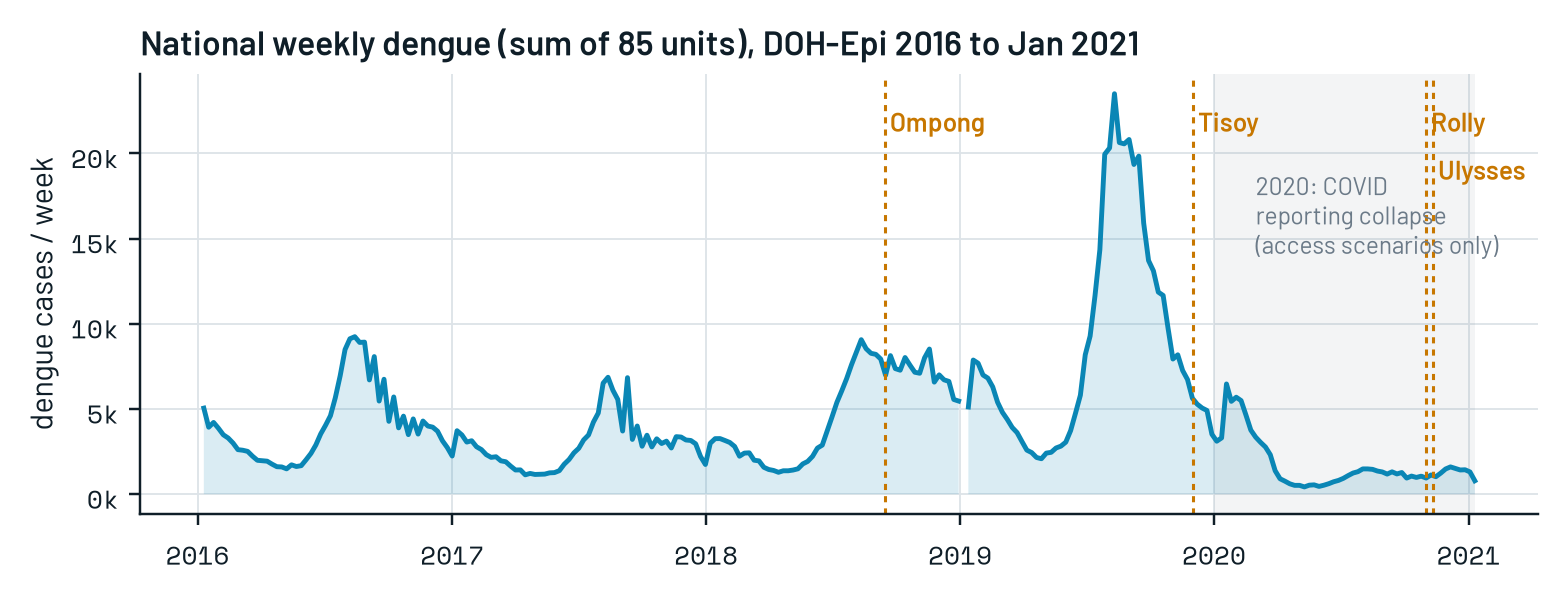
\includegraphics[width=\linewidth]{f01_timeline}
\caption{The forecast target: weekly dengue cases from the Department of Health (DOH), summed over the \nUnits{} harmonised units, with the four backtest typhoons. 2020 is used for access scenarios only.}
\label{fig:timeline}
\end{figure}
